% DOCUMENT SETUP
\documentclass[10pt,twoside]{book}                  %Official DTU-IMM Thesis document setup

	%Set to 'print' for printed version, use 'net' for online version
	\def\thesisversion{net}

	% PACKAGES
	\usepackage{dtu}                                   % Import Thesis base style
	%input{PhDMacros}                                  % Thesis specific macros
	\usepackage[linesnumbered,lined,boxed,commentsnumbered]{algorithm2e}						% options http://en.wikibooks.org/wiki/LaTeX/Algorithms 
	\usepackage{tikz-qtree}                            % DOM representation
	\usepackage{tabularx}                              % Page width table


	% THESIS PROPERTIES (Modifiy these fields with your details)
	\def\thesisauthor{Mantas Kanaporis}                     %Author
	\def\thesistitle{Optimizing Web Extraction Queries For Robustness}               %Title
	\def\thesishandin{15-January}                       %Submission date (Day-Month}
	\def\thesisdegree{M.Sc.}                              %Degree ('B.Eng', 'B.Sc.', 'M.Sc.' or 'PhD')
	\def\thesisyear{2015}                               %Submission year
	\def\thesisnumber{????}                             %DTU-IMM Serial number (do not include year)
	\def\thesisISSN{0000-0000}                          %ISSN number
	\def\thesiskeywords{Robust wrappers}  %PDF keywords
	\derivethesisprops                                  %Derive dependent properties

	% SECTION NUMBERING SETUP
	\setcounter{tocdepth}{2}                            %2 adds sections up to subsections
	\setcounter{secnumdepth}{3}                         %Subsubsections get a number when this is 3

% THESIS STRUCTURE  (Modifiy to include more chapters etc)
\begin{document}

	%Pre-frontmatter material
	\prefrontmatter

	%Frontmatter material
	\frontmatter
	\pagenumbering{roman}                               %Set frontmatter numbering style
	\chapter{Summary}

The web contains semi-structured information in HTML, i.e. tree structure. To extract semantic data from a web page, which gets updated, a non-breaking algorithm is required. Building the most robust wrapper is the subject of this project. Current state of the art proposes robust web extraction framework that uses archival data and training examples to build the wrapper. We constrain our problem by having a single base version of a web page, a single training example and limited execution time. Building on the framework, I would carry out an empirical research and experiment with variations: (1) precompute various minimum cost models, (2) try $O(n)$ heuristics for calculating min diff between two trees vs $O(n^3)$ traditional approach, (3) try different candidate wrapper generation techniques.
                                   %English summary of Thesis
	\markboth{}{}                                       %Set headings (left)(right)
	\chapter{Preface}

This thesis was prepared at the department of Informatics and Mathematical Modelling at the Technical University of Denmark in fulfilment of the requirements for acquiring an M.Sc. in Informatics.

The thesis deals with designing, implementing and testing a new method for robust record-level data extraction from web pages, given a single annotated page as a training set.

The thesis consists of three main parts: (1) the design of the algorithm, including state of the art method overview, (2) Java implementation of the design, and (3) an experiment, which tested performance and accuracy of the implementation with real world dataset.

%==================================================================================================
% SIGNATURE AREA
%==================================================================================================
\vspace{20mm}
\begin{center}
    \hspace{20mm} Lyngby, \thesishandin-\thesisyear
    \vspace{5mm}
    \newline
  %Update signature image file in line below
%    
\includegraphics[scale=0.25]{figures/signature}
\end{center}
\begin{flushright}
    \thesisauthor
\end{flushright}
% % % EOF % % %

% vim:wrap linebreak nolist:
                                     %Preface
	\markboth{}{}                                       %Set headings (left)(right)
	%\chapter{Acknowledgements}

I would like to thank my supervisor prof. Michael Reichhardt Hansen from the Technical University of Denmark and company representative Henrik Pilegaard from Kapow Software. I am really grateful for the trust and advice I have received.


% vim:wrap linebreak nolist:
                            %Acknowledgements
	%\markboth{}{}                                       %Set headings (left)(right)

	% Table of contents
	\newpage\mbox{}\newpage
	\chaptermark{Contents}
	\pdfbookmark{\contentsname}{toc}
	\renewcommand{\sectionmark}[1]{\markright{#1}}
	\sectionmark{Contents}
	\addtolength{\parskip}{-\baselineskip}
	\tableofcontents
	\addtolength{\parskip}{\baselineskip}
	\renewcommand{\sectionmark}[1]{\markright{\thesection\ #1}}
	
	% Main content
	\mainmatter
	\chapter{Introduction}

% Typically 4-7 pages.

\section{Background} % (fold)
\label{sec:Problem}

% Introduce the domain of information extraction.

The World Wide Web contains a vast amount of information, counting in billions of web pages \cite{signorini2005a}. Mostly it is unstructured or semi-structured documents, making it difficult to process the data directly by machines. As a result, sharing and reusing knowledge across multiple parties is hardly possible without human interaction.

Addressing the need to automatically extract and process large volumes of accessible information, machine needs to extract loosely-structured data from web sources and populate databases with well-structured data for further handling. The problem can be seen as information extraction problem for web pages. 

There are many use cases for sharing data between web-based applications with no dedicated integration capabilities. Some examples include extracting product price information from competitor on-line shops, or integrating with an online scheduling application which has no application programming interface (API). In both cases data is presented to the user via the web browser and no special care was taken to make it easy for automatic extraction.


\section{Problem}

% Since you have a goal, there must be some problem that you are trying to solve. Explain this problem. What people in the real world are affected by the problem that concerns you? It is best if your grandmother understands this section.

% Web wrapping
Most of the pages on the web are HTML documents. Many websites use view templates to generate individual pages on the server side. Thus, a list of objects on a page, generated by a template, has a repeating structural pattern. HTML has a tree structure and can be viewed as a labeled ordered rooted tree. To extract information from the webpage, one needs to query a node in a tree. The program that performs the actual information extraction (IE) task from webpages is called a \emph{web wrapper}. The web wrapper query can be expressed in a number of standartized notations, e.g. XPath, CSS selectors, etc.

% Robustness
For a webpage, writing a query that extracts a certain piece of information is a straight forward task. A query can be written in many ways and still uniquelly target the same node in document object model (DOM) tree. The problem gets really interesting when one takes into consideration that websites are maintained and evolve over time. A slight change of the HTML document structure might result in a non-functional wrapper.

% Data records
In this paper, we focus on web pages that contain a list of similar items, e.g. a list of products. These \emph{data records} are displayed in a web page with regular pattern. Figure~\ref{fig:amazon-books-html} provides an example, a part of the web page that lists four books. The full description of each book is a data record. The actual tag tree for the page in Figure~\ref{fig:amazon-books-html} is given in Figure~\ref{fig:amazon-books-tree}.

\begin{figure}
	\centering
	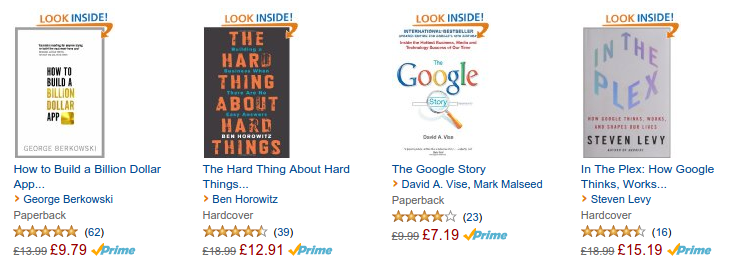
\includegraphics[width=1.0\textwidth]{figures/amazon-books}
	\caption{An example of four data records.}
	\label{fig:amazon-books-html}
\end{figure}

\begin{figure}
	\centering
	\Tree [.table 
			[.thead 
				[.tr 
					[.th [.\textit{Vorname} ] ]
					[.th [.\textit{Nachname} ] ]
				]
			]              
			[.tbody 
				[.tr 
					[.td [.\textit{Donald} ] ]
					[.td [.\textit{Duck} ] ]
					[. ... ]
				]
			]
		]
	\caption{Tag tree of the page in Figure~\ref{fig:amazon-books-html}}
	\label{fig:amazon-books-tree}
\end{figure}

\begin{figure}
	\centering
    \begin{tabularx}{\textwidth}{ | l | l | l | l | l | l | p{5cm} |}
		\hline
		\textbf{Title} & \textbf{Author} & \textbf{Cover} & \textbf{Comments} & \textbf{Old price} & \textbf{New price} \\ 
		\hline
		How to Build a Billion Dollar App ... & George Berkowski & Paperback & 62 & 13.99 & 9.79 \\ 
		\hline
		The Hard Thing About Hard Things ... & Ben Horowitz & Hardcover & 39 & 18.99 & 12.91 \\ 
		\hline
		The Google Story & David A. Vise, Mark Malseed & Paperback & 23 & 9.99 & 7.19 \\ 
		\hline
		In The Plex: How Google Thinks, Works ... & Steven Levy & Hardcover & 16 & 18.99 & 15.19 \\ 
		\hline
    \end{tabularx}
\end{figure}

% Annotation and automation
A \emph{record-level wrapper} extracts multiple records from a single web page, while a \emph{page-level wrapper} extracts a single piece of information from a page. Wrappers rely on extraction rules to identify the data field to be extracted. Most wrapper generation techniques learn the extraction rules from a training set. A user manually \emph{annotates} sample pages by pointing to tree nodes with relevant pieces of information.

% Subject of this paper
Building a robust and fast record-level wrapper from a single annotated web page within reasonable execution time is the subject of this paper. Defining wrapper \emph{robustness} is a problem of its own. Some format definitions will be shown later. Informally, it's the wrapper that has the lowest odds of breaking after any changes to the web page structure.

% Relevance
The problem of building a robust wrapper is relevant in many areas, inluding web application integration, web user interface test automation, and web scrapping.


\section{Goal}

% After the motivation (why) explain in detail what the goal is. If your project contains an element of research (which is good) the goal is more like a hypothesis. In other words, your goal is to investigate some particular method to verify its usefulness for some particular purpose (verify the hypothesis).

The goal of this thesis is to design and test an algorithm for building a robust and fast record-level wrapper from a single annotated HTML \emph{snapshot}, i.e. a specific document version at a given time. Futhermore, the algorithm is constrained with the following limitations and assumptions:

\begin{enumerate}
	\item There is a single annotated snapshot of a web page, i.e. training set of one.
	\item The wrapper must be robust and correctly extract information from the future web page versions.
	\item The wrapper must be reasonably fast on commodity hardware.
\end{enumerate}

Inputs: 

\begin{enumerate}
	\item $w_{base}$ -- An initial snapshot of annotated HTML document.
	\item $d(w_{base})$ -- A location of a single record attribute node in the annotated document.
	\item $w_{new}$ -- New (possibly updated) snapshot of the same HTML document.
\end{enumerate}

Outputs: 

\begin{enumerate}
	\item $\{a'_i\}$ -- Extracted attribute values of data records in a new document, e.g. book titles.
	\item $c$ -- \emph{Confidence} measure, i.e. the probability measure that the wrapper did not break. This shows how accurate was the extraction.
\end{enumerate}

The following example illustrates sample inputs and outputs. An initial snapshot $w_{base}$ of a sample HTML document is illustrated in Figure~\ref{fig:sample-tree}. The annotated attribute node $d(w_{base})$ is marked with parenthesis. The extracted record attribute values are $\{\text{Carol}, \text{Bob}, \text{Alice}\}$ with $90\%$ confidence.

\begin{figure}
	\centering
	\Tree [.table 
			[.thead 
				[.tr 
					[.th [.\textit{Name} ] ]
					[.th [.\textit{Age} ] ]
				]
			]              
			[.tbody 
				[.tr 
					[.td [.\textit{(Carol)} ] ]
					[.td [.\textit{18} ] ]
				]
				[.tr 
					[.td [.\textit{Bob} ] ]
					[.td [.\textit{19} ] ]
				]
				[.tr 
					[.td [.\textit{Alice} ] ]
					[.td [.\textit{20} ] ]
				]
			]
		]
	\Tree [.table 
			[.tr 
				[.td [.\textit{(Carol)} ] ]
				[.td [.\textit{18} ] ]
			]
			[.tr 
				[.td [.\textit{(Bob)} ] ]
				[.td [.\textit{19} ] ]
			]
			[.tr 
				[.td [.\textit{(Alice)} ] ]
				[.td [.\textit{20} ] ]
			]
		]
	\caption{An initial $w_{base}$ (on the left) and a transformed $w_{new}$ (on the right) snapshots of a sample HTML document. Distinguished nodes marked in paranthesis.}
	\label{fig:sample-tree}
\end{figure}



\section{Contribution}

% What methods are used?
% Briefly references to related research (just the main references – more references in chapter ”Related research” or throughout the thesis)
% Emphasize your own contribution: what is original or new?

In this paper, we present a new method for fast and robust record-level data extraction. The method builds on three lines of work and combines them in a novel way: \emph{data region mining} \cite{liu2009a} to recognize template generated areas on a web page, \emph{probabilistic wrapper induction} \cite{DBLP:journals/pvldb/ParameswaranDGR11} to extract data from a single data region in a robust way, and \emph{partial tree alignment} \cite{zhai2005a} to repeatedly extract data from multiple regions. 

% How each method work. How they are combined.
The main idea is to split wrapping process into two steps. First, we match the data region boundary. Next, we operate inside the boundary per each data record. We use a minimal tree-edit distance and a probabilistic HTML change model as primary tools for both steps. Eventually, we build a partial tree which is later used for attribute value extraction from multiple data regions. And pattern matching is used for content double checking.

% 1. Why did you choose to combine these three methods? Are there alternatives?
% 2. What can other methods do?

% Why? Alternatives? 
% Probabilistic wrapper induction
\cite{DBLP:journals/pvldb/ParameswaranDGR11} introduces the idea of computing edit-distance between two trees (or DOMs), formally defines robustness, and later designs a dynamic programming algorithm for finding the optimal wrapper. Most alternative wrapping techniques [TODO: refs] require large training sets, or use no formal definition of robustness. Yet the method is limited to extracting a single distinguished node from a tree. Thus, we consider it as a state of the art method.

% Why? Alternatives? 
% Data record mining
To enable wrapping in a web page with multiple data records, we need to locate individual data record regions and run page-level wrapper inside a single region. Thus we choose \cite{liu2009a} proposed technique for mining data regions. Unlike most alternatives [TODO: refs] this method ... We also experimented with method variations by implementing tree-edit distance instead of original string edit-distance. And also other optimiztions for our particular use-case.
String matching vs Probabilistic tree change model, which is more accurate

% Why? Alternatives? 
% Broom extraction

% 3. Why do you think that your method will be better? (This is in fact the thesis of your thesis.) You should elaborate a bit on each of these points. That is, relate your approach to the state-of-the-art and argue for your choice.
Data records on the web and probabilistic change models for trees have not been combined before into a coherent system. We demonstrate that our method is both accurate and fast. (more about the experiment setup and findings later) We also show that chosen techniques can be optimized / fine-tuned for specific use-case to get better performance and accuracy.

% TODO I suggest that you take a little concrete example and explain your method in terms of that, so that the reader can see the input HTML tree, what you use each of the three methods for, and what you get as result.


\subsection{Example: method in action}

The new method is best illustrated by an example.

A wrapper is built from original snapshot:

\begin{enumerate}
	\item A global wrapper is built to locate a distinguished node.
	\item Data regions on the original page are located.
	\item A broom is extracted from all regions.
	\item A local wrapper is built for single region.
\end{enumerate}

Wrapping process on the new snapshot:

\begin{enumerate}
	\item A candidate node is located in a new page with a global wrapper.
	\item Data regions on the original page are located.
	\item A local wrapper is run through each data region to extract data records.
\end{enumerate}


% What I managed to do, though, is to narrow down my focus to the tool-for-the-job – a tree edit-distance application. There are three recent papers that build on this idea \cite{DBLP:conf/sigmod/DalviBS09}, \cite{DBLP:journals/pvldb/ParameswaranDGR11}, \cite{DBLP:conf/wism/LiuWYL12}.

% While the idea of robust wrappering is not new, the core difference from earlier systems is the unique combination of ideas and tools that are optimized for performance.

% Here the idea of computing edit-distance between two trees (or DOMs) is introduced, robustness is defined formally, and later dynamic algorithm for finding the optimal wrapper is designed. My contribution was to implement the algorithm, optimize the performance using the latest research, and improve the algorithm to support multiple result sets (as opposed to single node from the query).

% I would carry out an empirical research and experiment with variations: (1) precompute various minimum cost models, (2) try $O(n)$ heuristics for calculating min diff between two trees vs $O(n^3)$ traditional approach, (3) try different candidate wrapper generation techniques.

% Build on the basis of \cite{DBLP:journals/pvldb/ParameswaranDGR11}, implement optimizations and run empirical experiments: (1) think of change probabilities model, (2) optimize for multiple extractions, (3) parallize with functional implementation, (4) analyze for multiple distinguished nodes extraction, (5) identify repeating elements of page + the base and run wrapper in each subtree of the base.

% We could compare various XPath enumeration techniques, eg Dalvi'09, vs Probabilistic model Parameswaran'11.

% Add visual features and content patterns to the structural model \cite{Chidlovskii:2006:DES:1142473.1142555}. (Visual features, which are obtained from web browsers API, enhance understanding of semantic similarity between web page elements.) Improve Parameswaran'11 with content models (see wrapper repairs).

% For multiple nodes per wrapper on same page, recognize data regions first Zhai and run all the wrapper inducers later. Utilize record-level wrapper induction \cite{DBLP:conf/cikm/ZhengSWG09}.

% According to (Myllymaki \& Jackson, 2002), robustness can be achieved by “relying less on page structure and more on content.” Use more of that. We think that in addition to this, the total number of hops should be minimized because every additional hop increases the risk of failure.

% Dalvi'09 on change model learning:
% - same set of tags appear in the top list for insertions and deletions, i.e. a, br tend to be be more volatile.
% - same sets of tags appear in the top of the list. most volatile tags may not depend heavilyt on the data?
% - yet tr,td are more prominent in some websites. also ul, li. depends on how layouts are made.


\section{Organization}

We define the main concepts of the problem domain in Chapter 2. In Chapter 3 we discuss current state of the art across relevant lines of research. Chapters 4-8 describe our method in detail and elaborate on the design decisions. We present the empirical experiment results in Chapter 9. The thesis is conluded with findings discussion and future research direction.


% vim: set wrap

	\chapter{Main concepts}

% Describe your own work (how you reached your goal) and take care to motivate your choices. Don't just describe all the things you did – tell us why.

\section{Labeled ordered rooted tree}
\section{Data records}

\section{Wrapper}

The term originates from information system integration domain \cite{Chang:2006:SWI:1159162.1159300}, where a proxy interface abstracts away the complexity of accessing a data source. 

\section{Wrapper robustness}
\section{Edit tree distance}
\section{Partial tree alignment}

% vim: set wrap

	\chapter{Related Work}

% You will need to describe what has been done before and you will need to discuss the theory that your work is based upon. This is a slightly dangerous: Take care not to punish the reader with hairy theory without explaining why it is needed.

% What is the main idea? What is the contribution (the new or interesting thing)? What is important for you? Where it is presented?

% Gist + My comment
% TODO: go through each paper and make short notes on what's important and why.

The method presented in this paper builds on the previous work in wrapper induction, HTML aware data extraction, probabilistic tree-edit distance measures, and data record mining. The most influential ideas are covered in chapter.


% ---------------------------------------------------------------------
\section{Wrapper Induction Method Overview}
% discuss classification and state our focus

The problem of data extraction (from web pages?) has been addressed in a number of papers. \cite{Laender:2002:BSW:565117.565137} reviews multiple techniques for generating wrappers, inluding natural language processing, languages and grammar, machine learning, information retrieval, databases, and ontologies. A common goal of all wrapper generation tools is to build a wrapper that is both accurate and robust, but is built with the least possible human interaction. The article provides a taxonomy for grouping wrapping techniques.

The most relevant category mentioned in the paper is the HTML-aware tools. These rely on structural features of HTML documents. The document is parsed into a tree structure and extraction rules are applied to the tree. Altough the tools discused (XWRAP, W4F, RoadRunner) provide a high degree of automation, many of them rely on heuristics and have a weak notion of robustness.

In a more recent overview of web data extraction techniques \cite{Chang:2006:SWI:1159162.1159300} the author argues, that due to template generated content, web IE problems can take advantage machine learning and pattern matching methods. Compare it to traditional IE approaches that are mostly based on natural language processing (NLP). Unsupervised approaches can only support template pages. The extension of such systems to non-template page extraction tasks is very limited.

As our research focus is data extraction from HTML documents which are semi-structured, we focus on techniques based on structural features rather than vague NLPs that require large training sets. Yet the content models are interesting direction for extra accuracy.

% TODO Liu
Several approaches have been reported in the literature for mining data records from Web pages.  There are two main types of algorithms, wrapper induction and automatic extraction. In wrapper induction [11, 19, 23, 25, 33], a set of extraction rules are learnt from a set of manually labeled pages or data records. These rules are then used to extract data items from similar pages. This method still requires substantial manual efforts. In automatic methods, [12][1] find patterns or grammars from multiple pages containing similar data records. Requiring an initial set of pages containing similar data records is, however, a major limitation of this type of approaches because such pages have to be found manually or by another system.

% ---------------------------------------------------------------------
\section{HTML Aware Data Extraction}
% elaborate on the research in the area of our focus

% IBM Report: Robust Web Data Extraction with XML Path Expressions
One the the first papers to discuss XPath based wrappers was \cite{Myllymaki02robustweb}. In this approach, XML tools are used convert HTML document into pure XHTML and XPath queries extract desired pieces of information. The wrapper is a set of XSLT extraction rules, i.e. hops that are based on structure, attributes, or content. Yet the actual XPath queries were written by hand without any automation.

The same paper mentions robustness as a feature of a good extraction rule. The author informally defines robustnes as the ability to extract intended data from an HTML page after structural changes to the page. Two metrics for measuring robustness are introduced. The first is a number of times that expression failed to extract correct results. The second is expression complexity in terms of depth. The paper defines a notion of anchors (DOM tree nodes) and hops (relative XPath expressions) over a normalized HTML document. 

% Relative vs absolute queries: Robust Web Contet Extraction
Some techniques \cite{Chang:2006:SWI:1159162.1159300} improve the robustness of XPath expression. The general approach of these techniques is to rewrite the expression into a more robust relative one by tracking structural changes in the traning set. \cite{Kowalkiewicz:2006:RWC:1135777.1135928} empirically confirmed that there is a notable difference between various versions of wrappers in terms of robustness – relative XPath expressions outperform absolute ones significantly. This proves the idea that some wrappers are more robust.

% Vertex tool
\cite{DBLP:conf/icde/GulhaneMMRRSSTT11} introduces apriori style algorithm for learning xpath-based extraction rules that are robust to variations in site structure. Algorithm learns rules from human annotated pages based on structural features. Based on domain knowledge, these features are classified into strong (e.g. HTML attributes \texttt{class} or \texttt{id}, tags, textual fragments) and weak (e.g. \texttt{font}, \texttt{width} attributes). This method tries to build a path from strong features only by generating and combining candidates. If Apriori fails to output precise XPath, Naive-Bayes based classifier is used to evaluate the best guess of newly generated nodes with weak features. Essentially this method is based on enumeration, which makes it slow for large websites. Additional limitations are the use of large training set and that it requires a set of annotated pages for certain heuristics (e.g. support metrics) to properly work. 

% WebSelF tool
\cite{Thomsen:2012:WWS:2364120.2364156} presents a framework that takes into account not only the structure and the content of a scrapped page, but also the context and the presentation, i.e. the location where the data is physically located after full rendering and applying stylesheets. It also works with dynamic page elements, that are frequent in JavaScript rich web pages. The design of the framework consists of three type of functions: for selecting elements, for for verifying the selected elements, and for maintaining the previous functions.

- http://www.cs.uic.edu/~liub/WebMiningBook.html\\


% ---------------------------------------------------------------------
\section{Tree-Edit Models}

% Zhang-Shasha edit-tree distance
To compare similarity of two HTML documents we can use string edit distance or tree edit distance. A distance between two labeled ordered rooted trees is considred to be the weighted number of edit operations (insert, edit, delete) to transform one tree into another \cite{shasha1990a}. The proposed algorithm to address the problem of finding the minimum set of operations to transform one tree into another has a complexity of $O(n_1 n_2 h_1 h_2)$, where $n_1$ and $n_2$ are the size of the trees, and $h_1$ and $h_2$ are heights of the trees.

% Automatic web news extraction using tree edit distance by Reis'04
In \cite{de2004a} author introduces \emph{Restricted Top-Down Mapping} algorithm, which calculates edit-tree distance by efficiently analysing tree structure. Generally, the algorithm imposes top-down mappings which allow removal and inserts at the bottom of the tree only. Informally, we expect some minor changes inside templates, i.e. just the content at the bottom of the elements.

% Broom analogy
The paper \cite{de2004a} instroduces the idea of tree extractor, i.e. tree structure with wildcards for matching HTML documents. This step recognizes common pattern between two trees. Basically, the template is reconstructed from multiple HTML fragments.

% TODO
- A Survey on Tree Edit Distance and Related Problems\\

% Edit cost / Change model
In \cite{de2004a} two tree similarity threshold as fixed constant of 80\%. Every vertex insertion, removal or replacement has unit cost of one. In \cite{dalvi2009a} the probability distribution of the next page state is based on structural patterns in the training set.

% TODO Rewrite [Dalvi'09]
A number of papers have focused on finding the edit distance, or shortest editing script that changes a source tree to a target tree (see [6] and citations). There are also weighted versions of tree edit distances that assign different weights to different edit operations. However, these models do not define a probability distribution: they do not compute the probability of a source tree changing to the target tree, but only the shortest/lightest path according to the weights. To see the difference, consider the two tree transformations of Figure 12. Clearly, each transformation has an edit distance of 1; in the first case, corresponding to deletion of the left- most L1 child, and in the second case corresponding to the deletion of any of the n nodes. Clearly, the second transformation is far more probable (if individual edits have the same probability). The lack of a probability distribution also makes it difficult to define a principled learning component that can learn the weights of various edit operations.

% TODO
- RTED - A Robust Algorithm for the Tree Edit Distance\\

% TODO
- Simple fast algorithms for the editing distance between trees and related problems\\

% TODO
- React’s diff algorithm\\

Probabilistic model allow to formalize robustness.

% [Dalvi'09] Robust Web Extraction - An Approach Based on a Probabilistic Tree-Edit Model
Dalvi et al. to view page evolution as a stochastic process, where individual edit operations (delete, insert and substitute) are picked by their probability \cite{dalvi2009a}. Probabilities are learnt from a training set. The author introduces algorithm for efficiently estimating the probability of one tree evolving into the other. In other words, provides a first formal definition of robustness. Generates a set of candidate XPath wrappers and selects the most robust one. The problem with this approach is that it picks the local optimum from a generated set, rather the provably global optimum.

% Robust web extraction framework
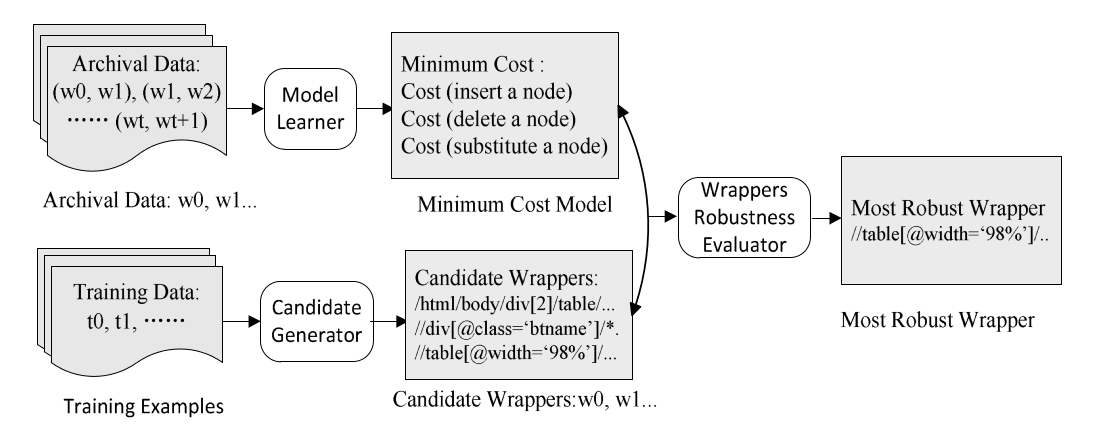
\includegraphics[width=\linewidth]{figures/robust-web-extraction-framework}

% [Parameswaran'11] Optimal Schemes for Robust Web Extraction
Building on prior work on formalizing wrapper robustness \cite{dalvi2009a}, Parameswaran et al. \cite{DBLP:journals/pvldb/ParameswaranDGR11} elaborate the concept of robustness and provides a method for building wrappers with provably optimal robustness. Two robustness models are introduced: the worst case and the most probable case. An algorithm for computing optimal wrapper is introduced of polinomial running time. Yet it is inefficient due to enumeration for computing the minimum cost scripts and extracting the distinguished node of interest \cite{DBLP:conf/wism/LiuWYL12}.


% ---------------------------------------------------------------------
\section{Data Record Mining}

\cite{liu2009a} proposes a Mining Data Records (MDR) algorithm for automatically locating data records in web pages. In other words, MDR finds page regions generated by a template. The method is based on edit distance string matching algorithm to find data records and two observations about data records in an HTML document. First, a group of data records have similar tree structure and are located in a close proximity. Second, these groups are under one parent node, i.e. it is very unlikely that a single record would begin inside one child subtree and end inside another child subtree. The algorithm works both with continous and non-continous data regions. The proposed method uses string matching rather than HTML tree structure, which is more accurate.

Building on Liu et al. work \cite{liu2009a}, Zhai and Liu further develops the idea of extracting data from a web page that contains several structured data records \cite{zhai2005a}. Their method is based on visual clues: style and position of elements after rendering. After identifying individual data records, the proposed approach aligns multiple tag trees into a generic \emph{seed tree}. The seed tree contains a maximum number of data record fields. (TODO: Elaborate) 

Similarly, in \cite{zheng2007a} the DOM tree is progressively converted into a generic page-level wrapper tree. A cost-driven dynamic programming is employed for the alignment algorithm. The issue with this approach is that tree-mapping operations are expensive. Zheng et al. further develop tree alignment idea \cite{DBLP:conf/cikm/ZhengSWG09} and introduce a concept of \emph{broom} structure, which effectively is a generalized record-level wrapper. By restricting alignment to relevant DOM regions, the tree alignment cost is reduced dramatically. It also handles case of cross records and uses content matching for improved record extraction.

% TODO
Both of the aforementioned tree alignment techniques are important for repeated record-level wrapping. This tree is an important structure to enable generalized wrapper for multiple record extraction.

Summary of pattern extraction. Automatic data extraction. Tree alignment to extract data by a template.

\paragraph{Automatic Wrappers for Large Scale Web Extraction.} Dictionaries and regular expressions. Content models?

% TODO rewrite as quoted from [REIS'04]
Bing Liu et al. have developed an effective algorithm for mining
data records from Web pages [14]. The algorithm has two steps.
In the first step it identifies the data region of the Web page and in
the second one it extracts the records themselves. The algorithm
works each time in a single page, so it does not compare the page
trees. Although achieving good results, the algorithm only works
with multi-record pages and therefore cannot be applied to on-line
news pages, that are almost exclusively single-record pages.

- 
% vim:wrap linebreak nolist:

	\chapter{Robust web extraction framework}

% Describe your own work (how you reached your goal) and take care to motivate your choices. Don't just describe all the things you did – tell us why.

HTML has a tree structure and can be viewed as an ordered labled tree.

Define the content more carefully: all sections and a brief description what you will write in each of them. Define the main concepts you will need and fix the notations. Then you can write the chapters in any order you want. Make also a work plan: what you will do and when.

Specify your topic carefully. Don’t take too large topic!  Invent a preliminary title for your thesis and define the content in a coarse level (main chapters). Ask your supervisor’s approval! Decide with your supervisor what material you should read or what experiments to make.  

You can write the thesis after you have read all material or made all experiments. However, you can begin to write some parts already when you are working. Often you have to change your design plan, but it is just life! Ask feedback from your supervisor, when your work proceeds.

\chapter{Generating minimal candidate wrappers}
\chapter{Learning edit costs}
\chapter{Building robust wrappers}
\chapter{Optimizing for performance with parallelization}


% vim: set wrap

	\chapter{Experiment evaluation}

This section should write itself. Since you have a goal, the results section must document that you have reached this goal (or verified your hypothesis).

\section{Experiment setup}
\subsection{Sample data}
\subsection{Distinguished nodes}
\subsection{Probabilistic change model}

\section{Implementation}

\section{Experiment results}

\section{Discussion}

% vim: set wrap

	\chapter{Conclusion}
% Just 1-3 pages!

You can conclude that you have reached your goal or discuss why not if that is the case. Also discuss hindsights: What things were even better or a little worse than expected regarding the methods you used to solve your problems. How could your project be improved by further work.

\section{Summary}

\section{Conclusion}

\section{Future research} % (fold)
\label{sec:section name}

% section section name (end)

% vim: set wrap


	% Appendixes
	\appendix
	\chapter{Source Code}
\label{ch:source}

% Include the code in Appendices and organize into some natural sections, so that you can refer to sections in the appendix from the main part of the thesis. If these are some non-trivial steps from your main thesis sections (Design and algorithms) to the actual implementation in the Appendix, then you could address these particular important implementation points in the thesis.

This appendix is contains the source code of the wrapper organized into sections by Java package names. The code listings do not include unit tests, which can be found in an online source repository at \url{https://bitbucket.org/mantiniss/thesis-wrapper}.


%----------------------------
\section{lt.kanaporis.thesis}
\subsection{lt.kanaporis.thesis.Config}
\lstinputlisting{source/Config.java}


%---------------------------------------
\section{lt.kanaporis.thesis.changemodel}

\subsection{lt.kanaporis.thesis.changemodel.NumberUtils}
\lstinputlisting{source/changemodel/NumberUtils.java}

\subsection{lt.kanaporis.thesis.changemodel.ProbabilisticChangeModel}
\lstinputlisting{source/changemodel/ProbabilisticChangeModel.java}

\subsection{lt.kanaporis.thesis.changemodel.ProbabilisticTransducer}
\lstinputlisting{source/changemodel/ProbabilisticTransducer.java}

\subsection{lt.kanaporis.thesis.changemodel.TransformationProbabilities}
\lstinputlisting{source/changemodel/TransformationProbabilities.java}


%---------------------------------------
\section{lt.kanaporis.thesis.html}

\subsection{lt.kanaporis.thesis.html.HtmlRecordWrapper}
\lstinputlisting{source/html/HtmlRecordWrapper.java}

\subsection{lt.kanaporis.thesis.html.HtmlTreeFactory}
\lstinputlisting{source/html/HtmlTreeFactory.java}

\subsection{lt.kanaporis.thesis.html.ProbabilisticChangeModelFactory}
\lstinputlisting{source/html/ProbabilisticChangeModelFactory.java}


%---------------------------------------
\section{lt.kanaporis.thesis.region}

\subsection{lt.kanaporis.thesis.region.DataRegion}
\lstinputlisting{source/region/DataRegion.java}

\subsection{lt.kanaporis.thesis.region.DataRegionLocator}
\lstinputlisting{source/region/DataRegionLocator.java}

\subsection{lt.kanaporis.thesis.region.DiffsToNextGeneralizedNode}
\lstinputlisting{source/region/DiffsToNextGeneralizedNode.java}


%---------------------------------------
\section{lt.kanaporis.thesis.tree}

\subsection{lt.kanaporis.thesis.tree.Forest}
\lstinputlisting{source/tree/Forest.java}

\subsection{lt.kanaporis.thesis.tree.Node}
\lstinputlisting{source/tree/Node.java}

\subsection{lt.kanaporis.thesis.tree.PostOrderNavigator}
\lstinputlisting{source/tree/PostOrderNavigator.java}

\subsection{lt.kanaporis.thesis.tree.RtedMapper}
\lstinputlisting{source/tree/RtedMapper.java}

\subsection{lt.kanaporis.thesis.tree.Tree}
\lstinputlisting{source/tree/Tree.java}

\subsection{lt.kanaporis.thesis.tree.TreeUtils}
\lstinputlisting{source/tree/TreeUtils.java}


%---------------------------------------
\section{lt.kanaporis.thesis.wrapper}

\subsection{lt.kanaporis.thesis.wrapper.ProbabilisticPageLevelWrapper}
\lstinputlisting{source/wrapper/ProbabilisticPageLevelWrapper.java}

\subsection{lt.kanaporis.thesis.wrapper.ProbabilisticRecordLevelWrapper}
\lstinputlisting{source/wrapper/ProbabilisticRecordLevelWrapper.java}


% vim:wrap linebreak nolist:

	
	% Backmatter
	\backmatter
	\chaptermark{Bibliography}
	\renewcommand{\sectionmark}[1]{\markright{#1}}
	\sectionmark{Bibliography}
	\addcontentsline{toc}{chapter}{Bibliography}        %Force addition of Bibliography to TOC
	\bibliographystyle{alpha}                           %Use alpha codes for references
	\bibliography{references}                           %Bibliography file called

\end{document}
